\documentclass[10pt]{article}
\usepackage[polish]{babel}
\usepackage[utf8]{inputenc}
\usepackage[T1]{fontenc}
\usepackage{amsmath}
\usepackage{amsfonts}
\usepackage{amssymb}
\usepackage[version=4]{mhchem}
\usepackage{stmaryrd}
\usepackage{multirow}
\usepackage{graphicx}
\usepackage[export]{adjustbox}
\graphicspath{ {./images/} }
\usepackage{bbold}

\begin{document}
\section*{EGZAMIN MATURALNY}
\section*{W ROKU SZKOLNYM 2017/2018}
\section*{MATEMATYKA}
\section*{POZIOM PODSTAWOWY}
FORMUŁA OD 2015\\
(„NOWA MATURA")

ZASADY OCENIANIA ROZWIĄZAŃ ZADAŃ\\
ARKUSZ MMA-P1

\section*{Zadania zamknięte}
Punkt przyznaje się za wskazanie poprawnej odpowiedzi (zaznaczenie wtaściwego pola na karcie odpowiedzi).

Zadanie 1. (0-1)

\begin{center}
\begin{tabular}{|l|l|c|c|}
\hline
\multicolumn{1}{|c|}{Wymagania ogólne} & \multicolumn{1}{|c|}{Wymagania szczegółowe} & \multicolumn{2}{|c|}{\begin{tabular}{c}
Poprawna \\
odp. (1 p.) \\
\end{tabular}} \\
\hline
\begin{tabular}{l}
II. Wykorzystanie \\
i interpretowanie \\
reprezentacji. \\
\end{tabular} & \begin{tabular}{l}
1. Liczby rzeczywiste. Zdajacy wykorzystuje \\
definicję logarytmu i stosuje w obliczeniach \\
wzory na logarytm iloczynu, logarytm ilorazu \\
\end{tabular} & \begin{tabular}{c}
Wersja \\
I \\
\end{tabular} & \begin{tabular}{c}
Wersja \\
i logarytm poteqgi o wykładniku naturalnym \\
(1.6). \\
\end{tabular} \\
\cline{3-4}
 & B & D &  \\
\hline
\end{tabular}
\end{center}

Zadanie 2. (0-1)

\begin{center}
\begin{tabular}{|l|l|c|c|}
\hline
\begin{tabular}{l}
II. Wykorzystanie \\
i interpretowanie \\
reprezentacji. \\
\end{tabular} & \begin{tabular}{l}
1. Liczby rzeczywiste. Zdający posługuje \\
się w obliczeniach pierwiastami dowolnego \\
stopnia i stosuje prawa działan na \\
pierwiastkach (1.3). \\
\end{tabular} & \begin{tabular}{c}
Wersja \\
I \\
\end{tabular} & \begin{tabular}{c}
Wersja \\
II \\
\end{tabular} \\
\cline{3-4}
 & C & A &  \\
\hline
\end{tabular}
\end{center}

Zadanie 3. (0-1)\\
II. Wykorzystanie i interpretowanie reprezentacji.

\begin{enumerate}
  \item Liczby rzeczywiste. Zdający oblicza potęgi o wykładnikach wymiernych i stosuje prawa działań na potęgach o wykładnikach wymiernych (1.4).
\end{enumerate}

\begin{center}
\begin{tabular}{|c|c|}
\hline
\begin{tabular}{c}
Wersja \\
I \\
\end{tabular} & \begin{tabular}{c}
Wersja \\
II \\
\end{tabular} \\
\hline
C & D \\
\hline
\end{tabular}
\end{center}

\section*{Zadanie 4. (0-1)}
\begin{center}
\begin{tabular}{|l|l|c|c|}
\hline
\begin{tabular}{l}
III. Modelowanie \\
matematyczne. \\
\end{tabular} & \begin{tabular}{l}
1. Liczby rzeczywiste. Zdający wykonuje \\
obliczenia procentowe, oblicza podatki, zysk \\
z lokat (1.9). \\
\end{tabular} & \begin{tabular}{c}
Wersja \\
$\mathbf{I}$ \\
\end{tabular} & \begin{tabular}{c}
Wersja \\
II \\
\end{tabular} \\
\cline { 3 - 4 }
 & C & A &  \\
\hline
\end{tabular}
\end{center}

Zadanie 5. (0-1)

\begin{center}
\begin{tabular}{|l|l|c|c|}
\hline
\multirow{2}{*}{\begin{tabular}{l}
I. Wykorzystanie \\
i tworzenie informacji \\
\end{tabular}} & \begin{tabular}{l}
3. Równania i nierówności. Zdający \\
rozwiązuje nierówności pierwszego stopnia \\
z jedną niewiadomą (3.3). \\
\end{tabular} & \begin{tabular}{c}
Wersja \\
$\mathbf{I}$ \\
\end{tabular} & \begin{tabular}{c}
Wersja \\
II \\
\end{tabular} \\
\cline { 3 - 4 }
 & $\mathbf{A}$ & $\mathbf{C}$ &  \\
\hline
\end{tabular}
\end{center}

Zadanie 6. (0-1)\\
$\left.\begin{array}{|l|l|c|c|}\hline & \begin{array}{l}\text { 4. Funkcje. Zdający interpretuje } \\ \text { I. Wykorzystanie } \\ \text { i tworzenie informacji }\end{array} & \begin{array}{l}\text { współczynniki występujace we wzorze funkcji } \\ \text { kwadratowej w postaci kanonicznej, w postaci } \\ \text { ogólnej i w postaci iloczynowej (o ile istnieje) } \\ \text { (4.10). }\end{array} & \begin{array}{c}\text { Wersja } \\ \text { I }\end{array}\end{array} \begin{array}{c}\text { Wersja } \\ \text { II }\end{array}\right]$

\section*{Zadanie 7. (0-1)}
\begin{center}
\begin{tabular}{|l|l|c|c|}
\hline
\multirow{3}{*}{\begin{tabular}{l}
I. Wykorzystanie \\
i tworzenie informacji \\
\end{tabular}} & \begin{tabular}{l}
3. Równania i nierówności. Zdający \\
rozwiązuje proste równania wymierne, \\
prowadzące do równań liniowych lub \\
kwadratowych (3.8). \\
\end{tabular} & \begin{tabular}{c}
Wersja \\
I \\
\end{tabular} & \begin{tabular}{c}
Wersja \\
II \\
\end{tabular} \\
\cline { 3 - 4 }
 & D & B &  \\
\hline
\end{tabular}
\end{center}

\section*{Zadanie 8. (0-1)}
\begin{center}
\begin{tabular}{|l|l|c|c|}
\hline
\multirow{3}{*}{\begin{tabular}{l}
I. Wykorzystanie \\
i tworzenie informacji. \\
\end{tabular}} & \begin{tabular}{l}
4. Funkcje. Zdajaccy interpretuje \\
współczynniki występujące we wzorze funkcji \\
liniowej (4.7). \\
\end{tabular} & \begin{tabular}{c}
Wersja \\
I \\
\end{tabular} & \begin{tabular}{c}
Wersja \\
II \\
\end{tabular} \\
\cline { 3 - 4 }
 & D & B &  \\
\hline
\end{tabular}
\end{center}

Zadanie 9. (0-1)

\begin{center}
\begin{tabular}{|l|l|c|c|}
\hline
\multirow{3}{*}{\begin{tabular}{l}
II. Wykorzystanie \\
i interpretowanie \\
reprezentacji. \\
\end{tabular}} & \begin{tabular}{l}
4. Funkcje. Zdajaccy szkicuje wykres funkcji \\
kwadratowej, korzystając z jej wzoru (4.8). \\
\end{tabular} & \begin{tabular}{c}
Wersja \\
I \\
\end{tabular} & \begin{tabular}{c}
Wersja \\
II \\
\end{tabular} \\
\cline { 3 - 4 }
 &  & C & D \\
\hline
\end{tabular}
\end{center}

Zadanie 10. (0-1)

\begin{center}
\begin{tabular}{|l|l|c|c|}
\hline
\begin{tabular}{l}
I. Wykorzystanie \\
i tworzenie informacji \\
\end{tabular} & \begin{tabular}{l}
4. Funkcje. Zdajacy wyznacza wzór funkcji \\
liniowej na podstawie informacji o funkcji lub \\
o jej wykresie (4.6). \\
\end{tabular} & \begin{tabular}{c}
Wersja \\
I \\
\end{tabular} & \begin{tabular}{c}
Wersja \\
II \\
\end{tabular} \\
\cline { 3 - 4 }
 & D & A &  \\
\hline
\end{tabular}
\end{center}

Zadanie 11. (0-1)

\begin{center}
\begin{tabular}{|l|l|c|c|}
\hline
\multirow{3}{l}{\begin{tabular}{l}
III. Modelowanie \\
matematyczne. \\
\end{tabular}} & \begin{tabular}{l}
5. Ciągi. Zdający bada, czy dany ciąg jest \\
arytmetyczny lub geometryczny (5.2). \\
\end{tabular} & \begin{tabular}{c}
Wersja \\
I \\
\end{tabular} & \begin{tabular}{c}
Wersja \\
II \\
\end{tabular} \\
\cline { 3 - 4 }
 &  & $\mathbf{A}$ & $\mathbf{B}$ \\
\hline
\end{tabular}
\end{center}

Zadanie 12. (0-1)\\
$\left.\begin{array}{|l|l|c|c|}\hline \text { III. Modelowanie } \\ \text { matematyczne. }\end{array} \begin{array}{l}\text { 5. Ciągi. Zdający stosuje wzór na } n \text {-ty wyraz } \\ \text { i na sumę } n \text { początkowych wyrazów ciągu } \\ \text { arytmetycznego (5.3). }\end{array} \begin{array}{c}\text { Wersja } \\ \text { I }\end{array} \begin{array}{c}\text { Wersja } \\ \text { II }\end{array}\right]$

Zadanie 13. (0-1)

\begin{center}
\begin{tabular}{|l|l|c|c|}
\hline
\begin{tabular}{l}
III. Modelowanie \\
matematyczne. \\
\end{tabular} & \begin{tabular}{l}
5. Ciągi. Zdający stosuje wzór na $n$-ty wyraz \\
i na sumę $n$ początkowych wyrazów ciągu \\
geometrycznego (5.4). \\
\end{tabular} & \begin{tabular}{c}
Wersja \\
I \\
\end{tabular} & \begin{tabular}{c}
Wersja \\
II \\
\end{tabular} \\
\cline { 3 - 4 }
 & B & A &  \\
\hline
\end{tabular}
\end{center}

\section*{Zadanie 14. (0-1)}
\begin{center}
\begin{tabular}{|l|l|c|c|}
\hline
\multirow{2}{*}{\begin{tabular}{l}
II. Wykorzystanie \\
i interpretowanie \\
reprezentacji. \\
\end{tabular}} & \begin{tabular}{l}
6. Trygonometria. Zdający korzysta \\
z przybliżonych wartości funkcji \\
trygonometrycznych - odczytanych z tablic \\
(6.2). \\
\end{tabular} & \begin{tabular}{c}
Wersja \\
I \\
\end{tabular} & \begin{tabular}{c}
Wersja \\
II \\
\end{tabular} \\
\cline{3-4}
 & C & D &  \\
\hline
\end{tabular}
\end{center}

Zadanie 15. (0-1)

\begin{center}
\begin{tabular}{|l|l|c|c|}
\hline
\multirow{2}{*}{\begin{tabular}{l}
I. Wykorzystanie \\
i tworzenie informacji. \\
\end{tabular}} & \begin{tabular}{l}
7. Planimetria. Zdający rozpoznaje trójkąty \\
podobne i wykorzystuje cechy podobieństwa \\
trójkątów (7.3). \\
\end{tabular} & \begin{tabular}{c}
Wersja \\
I \\
\end{tabular} & \begin{tabular}{c}
Wersja \\
II \\
\end{tabular} \\
\cline { 3 - 4 }
 & A & C &  \\
\hline
\end{tabular}
\end{center}

Zadanie 16. (0-1)

\begin{center}
\begin{tabular}{|l|l|c|c|}
\hline
\multirow{2}{*}{\begin{tabular}{l}
IV. Użycie i tworzenie \\
strategii. \\
\end{tabular}} & \begin{tabular}{l}
7. Planimetria. Zdają̧a stosuje zależności \\
między kątem środkowym i kątem wpisanym \\
(7.1). \\
\end{tabular} & \begin{tabular}{c}
Wersja \\
I \\
\end{tabular} & \begin{tabular}{c}
Wersja \\
II \\
\end{tabular} \\
\cline { 3 - 4 }
 & A & B &  \\
\hline
\end{tabular}
\end{center}

Zadanie 17. (0-1)

\begin{center}
\begin{tabular}{|c|c|c|c|}
\hline
\multirow[t]{2}{*}{III. Modelowanie matematyczne.} & \multirow[t]{2}{*}{7. Planimetria. Zdający korzysta z własności funkcji trygonometrycznych w łatwych obliczeniach geometrycznych (7.4).} & Wersja I & Wersja II \\
\hline
 &  & B & D \\
\hline
\end{tabular}
\end{center}

Zadanie 18. (0-1)

\begin{center}
\begin{tabular}{|l|l|c|c|}
\hline
\multirow{2}{*}{\begin{tabular}{l}
II. Wykorzystanie \\
i interpretowanie \\
reprezentacji. \\
\end{tabular}} & \begin{tabular}{l}
8. Geometria na płaszczyźnie kartezjańskiej. \\
Zdający wyznacza współrzędne środka \\
odcinka (8.5). \\
\end{tabular} & \begin{tabular}{c}
Wersja \\
I \\
\end{tabular} & \begin{tabular}{c}
Wersja \\
II \\
\end{tabular} \\
\cline { 3 - 4 }
 & B & A &  \\
\hline
\end{tabular}
\end{center}

Zadanie 19. (0-1)

\begin{center}
\begin{tabular}{|l|l|c|c|}
\hline
\multirow{2}{*}{\begin{tabular}{l}
II. Wykorzystanie \\
i interpretowanie \\
reprezentacji. \\
\end{tabular}} & \begin{tabular}{l}
8. Geometria na płaszczyźnie kartezjańskiej. \\
Zdający bada równoległość i prostopadłość \\
\end{tabular} & \begin{tabular}{c}
Wersja \\
I \\
\end{tabular} & \begin{tabular}{c}
Wersja \\
iI \\
kiestych na podstawie ich równań \\
\end{tabular} \\
\cline { 3 - 4 }
 & B & C &  \\
\hline
\end{tabular}
\end{center}

Zadanie 20. (0-1)

\begin{center}
\begin{tabular}{|l|l|c|c|}
\hline
 & \begin{tabular}{l}
II. Wykorzystanie \\
i interpretowanie \\
reprezentacji. \\
\end{tabular} & \begin{tabular}{l}
2. Stereometria. Zdający rozpoznaje \\
w graniastosłupach i ostrosłupach kąty między \\
odcinkami (np. krawędziami, krawędziami \\
i przekątnymi, itp.), oblicza miary tych kątów \\
\end{tabular} & \begin{tabular}{c}
Wersja \\
I \\
\end{tabular} \\
\hline
\end{tabular}
\end{center} \begin{tabular}{c}
Wersja \\
II \\
(9.1). \\
\end{tabular}

Zadanie 21. (0-1)

\begin{center}
\begin{tabular}{|c|c|c|c|}
\hline
\multirow[t]{2}{*}{II. Wykorzystanie i interpretowanie reprezentacji.} & \multirow[t]{2}{*}{9. Stereometria. Zdający rozpoznaje w graniastosłupach i ostrosłupach kąt między odcinkami i płaszczyznami (między krawędziami i ścianami, przekątnymi i ścianami), oblicza miary tych kątów (9.2).} & Wersja I & Wersja II \\
\hline
 &  & A & C \\
\hline
\end{tabular}
\end{center}

Zadanie 22. (0-1)

\begin{center}
\begin{tabular}{|l|l|c|c|}
\hline
\multirow{2}{*}{\begin{tabular}{l}
II. Wykorzystanie \\
i interpretowanie \\
reprezentacji. \\
\end{tabular}} & \begin{tabular}{l}
G11. Bryły. Zdający oblicza pole powierzchni \\
i objętość walca, stożka, kuli (G11.2). \\
\end{tabular} & \begin{tabular}{c}
Wersja \\
I \\
\end{tabular} & \begin{tabular}{c}
Wersja \\
II \\
\end{tabular} \\
\cline { 3 - 4 }
 &  & A & C \\
\hline
\end{tabular}
\end{center}

Zadanie 23. (0-1)

\begin{center}
\begin{tabular}{|l|l|c|c|}
\hline
 & \begin{tabular}{l}
10. Elementy statystyki opisowej. Teoria \\
prawdopodobieństwa i kombinatoryka. \\
II. Wykorzystanie \\
i interpretowanie \\
reprezentacji. \\
\end{tabular} & \begin{tabular}{l}
Zdający oblicza średnia ważoną i odchylenie \\
standardowe zestawu danych (także \\
\end{tabular} & \begin{tabular}{c}
Wersja \\
I \\
\end{tabular} \\
\cline { 3 - 4 }
 & \begin{tabular}{l}
Wersja \\
w przypadku danych odpowiednio \\
pogrupowanych), interpretuje te parametry dla \\
danych empirycznych (10.1). \\
\end{tabular} & B & D \\
\hline
\end{tabular}
\end{center}

Zadanie 24. (0-1)\\
\$\textbackslash left.\[
\begin{array}{|l|l|c|c|}\hline & \begin{array}{l}\text { 10. Elementy statystyki opisowej. Teoria } \\
\text { prawdopodobieństwa i kombinatoryka. } \\
\text { III. Modelowanie } \\
\text { matematyczne. }\end{array} & \begin{array}{l}\text { Zdający zlicza obiekty w prostych sytuacjach } \\
\text { kombinatorycznych, niewymagajacych użycia } \\
\text { wzorów kombinatorycznych, stosuje regułę } \\
\text { mnożenia i regułę dodawania (10.2). }\end{array} & \begin{array}{c}\text { Wersja } \\
\text { I }\end{array}\end{array}
\] \textbackslash begin\{array\}\{c\}\text{Wersja} \\


\text{II}\textbackslash end\{array\}\textbackslash right]\$ D \begin{tabular}{c}
B \\
\hline
\end{tabular}

Zadanie 25. (0-1)

\begin{center}
\begin{tabular}{|l|l|c|c|}
\hline
 & \begin{tabular}{l}
10. Elementy statystyki opisowej. Teoria \\
III. Modelowanie \\
matematyczne. \\
\end{tabular} & \begin{tabular}{l}
prawdopodobieństwa i kombinatoryka. \\
Zdający oblicza prawdopodobieństwa \\
w prostych sytuacjach, stosując klasyczną \\
definicję prawdopodobieństwa (10.3). \\
\end{tabular} & \begin{tabular}{c}
Wersja \\
I \\
\end{tabular} \\
\cline{3-4}
 & Wersja & II &  \\
\hline
\end{tabular}
\end{center}

\section*{Ogólne zasady oceniania zadań otwartych}
Uwaga: Akceptowane sa wszystkie odpowiedzi merytorycznie poprawne i spetniajace warunki zadania.

\section*{Zadanie 26. (0-2)}
II. Wykorzystanie i interpretowanie reprezentacji.\\
3. Równania i nierówności. Zdający rozwiązuje nierówności kwadratowe z jedną niewiadomą (3.5).

\section*{Przykładowe rozwiązanie}
Rozwiązanie nierówności kwadratowej składa się z dwóch etapów.\\
Pierwszy etap to wyznaczenie pierwiastków trójmianu kwadratowego $2 x^{2}-3 x-5$.\\
Drugi etap to zapisanie zbioru rozwiązań nierówności kwadratowej.\\
Pierwszy etap rozwiązania może zostać zrealizowany następująco:

\begin{itemize}
  \item zapisujemy nierówność w postaci $2 x^{2}-3 x-5>0$ i obliczamy pierwiastki trójmianu kwadratowego $2 x^{2}-3 x-5$
  \item obliczamy wyróżnik tego trójmianu:
\end{itemize}

$$
\Delta=9-4 \cdot 2 \cdot(-5)=49 \text { i stąd } x_{1}=\frac{3-7}{4}=-1 \text { oraz } x_{2}=\frac{3+7}{4}=\frac{5}{2}
$$

albo

\begin{itemize}
  \item stosujemy wzory Viète'a:
\end{itemize}

$$
x_{1} \cdot x_{2}=-\frac{5}{2} \text { oraz } x_{1}+x_{2}=\frac{3}{2}, \text { stą } x_{1}=-1 \text { oraz } x_{2}=\frac{5}{2} .
$$

Drugi etap rozwiązania: podajemy zbiór rozwiązań nierówności: $(-\infty,-1) \cup\left(\frac{5}{2},+\infty\right)$ lub $x \in(-\infty,-1) \cup\left(\frac{5}{2},+\infty\right)$.

\section*{Schemat punktowania \\
 Zdający otrzymuje}
gdy:

\begin{itemize}
  \item zrealizuje pierwszy etap rozwiązania i na tym zakończy lub błędnie zapisze zbiór rozwiązań nierówności, np.
  \item obliczy lub poda pierwiastki trójmianu kwadratowego $x_{1}=-1$ i $x_{2}=\frac{5}{2}$ i na tym zakończy lub błędnie zapisze zbiór rozwiązań nierówności,
  \item zaznaczy na wykresie miejsca zerowe funkcji $f(x)=2 x^{2}-3 x-5$ i na tym zakończy lub błędnie zapisze zbiór rozwiązań nierówności\\
albo
  \item realizując pierwszy etap popełni błędy, ale otrzyma nierówność, w której po jednej stronie występuje pełny trójmian kwadratowy posiadający dwa różne pierwiastki i konsekwentnie do popełnionych błędów wyznaczy zbiór rozwiązań nierówności.\\
Zdający otrzymuje 2 p.\\
gdy:
  \item poda zbiór rozwiązań nierówności: $(-\infty,-1) \cup\left(\frac{5}{2},+\infty\right)$ lub $x \in(-\infty,-1) \cup\left(\frac{5}{2},+\infty\right)$, lub $x<-1 \vee x>\frac{5}{2}$\\
albo
  \item poda zbiór rozwiązań nierówności w postaci graficznej z poprawnie zaznaczonymi końcami przedziałów\\
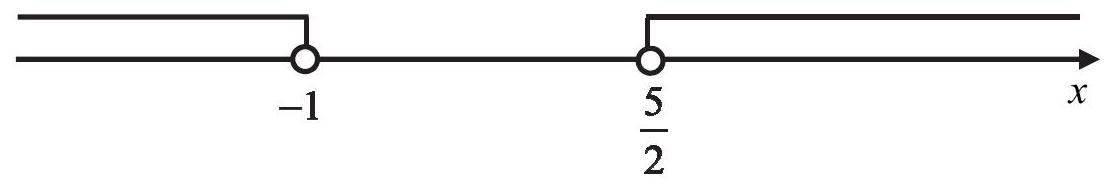
\includegraphics[max width=\textwidth, center]{2025_02_07_a74eed68a1a2147a06fdg-07}
\end{itemize}

\section*{Uwagi}
\begin{enumerate}
  \item Jeżeli zdający wyznacza pierwiastki trójmianu kwadratowego w przypadku, gdy obliczony wyróżnik $\Delta$ jest ujemny, to otrzymuje 0 punktów za całe rozwiązanie.
  \item Jeżeli zdający podaje pierwiastki bez związku z trójmianem kwadratowym z zadania, to oznacza, że nie podjął realizacji 1. etapu rozwiązania i w konsekwencji otrzymuje 0 punktów za całe rozwiązanie.
  \item Akceptujemy zapisanie odpowiedzi w postaci: $x<-1$ i $x>\frac{5}{2}, x<-1$ oraz $x>\frac{5}{2}$, itp.
  \item Jeżeli zdający poprawnie obliczy pierwiastki trójmianu $x_{1}=-1, x_{2}=\frac{5}{2}$ i błędnie zapisze odpowiedź, np. $x \in(-\infty, 1) \cup\left(\frac{5}{2},+\infty\right)$, popełniając tym samym błąd przy przepisywaniu jednego z pierwiastków, to otrzymuje 2 punkty.
  \item Jeżeli zdający po poprawnym rozwiązaniu nierówności zapisuje w odpowiedzi, jako zbiór rozwiązań, zbiór, zawierający elementy nienależące do zbioru $(-\infty,-1) \cup\left(\frac{5}{2},+\infty\right)$ lub zbiór pusty, to otrzymuje 1 punkt. Zapisanie w miejscu przeznaczonym na odpowiedź pierwiastków trójmianu kwadratowego nie jest traktowane jak opis zbioru rozwiązań.
\end{enumerate}

\section*{Kryteria uwzględniające specyficzne trudności w uczeniu się matematyki}
Jeśli zdający pomyli porządek liczb na osi liczbowej, np. zapisze zbiór rozwiązań nierówności w postaci $\left(-\infty, \frac{5}{2}\right) \cup(-1,+\infty),\left(+\infty, \frac{5}{2}\right) \cup(-1,-\infty)$, to przyznajemy 2 punkty.

\section*{Zadanie 27. (0-2)}
I. Wykorzystanie\\
i tworzenie informacji.\\
3. Równania i nierówności. Zdający korzysta z własności iloczynu przy rozwiązywaniu równań typu $x(x+1)(x-7)=0$ (3.7).

\section*{Przykładowe rozwiązanie}
Lewa strona równania jest iloczynem dwóch czynników $x^{3}+125$ oraz $x^{2}-64$. Zatem iloczyn ten jest równy 0 , gdy co najmniej jeden $z$ tych czynników jest równy 0 , czyli $x^{3}+125=0$ lub $x^{2}-64=0$.\\
Rozwiązaniem równania $x^{3}+125=0$ jest $x=\sqrt[3]{-125}=-5$.\\
Równanie $x^{2}-64=0$ doprowadzamy do postaci $(x-8) \cdot(x+8)=0$. Przynajmniej jeden z czynników $x-8$ lub $x+8$ jest równy 0 , czyli $x=8$ lub $x=-8$.

Równanie $\left(x^{3}+125\right)\left(x^{2}-64\right)=0$ ma trzy rozwiązania rzeczywiste: $x=-5, x=8 . x=-8$.

\section*{Schemat punktowania}
Zdający otrzymuje\\
gdy:

\begin{itemize}
  \item zapisze dwa równania $x^{3}+125=0$ i $x^{2}-64=0$\\
lub
  \item wyznaczy poprawnie (lub poda) rozwiązania jednego z równań: $x^{3}+125=0$ lub $x^{2}-64=0$\\
i na tym zakończy lub dalej popełni błędy.
\end{itemize}

\section*{Zdający otrzymuje \\
 gdy wyznaczy wszystkie rozwiązania równania: $x=-5, x=8, x=-8$.}
\section*{Uwagi}
\begin{enumerate}
  \item Jeżeli zdający poda wszystkie rozwiązania równania, bez rachunków lub uzasadnienia, to otrzymuje 2 punkty.
  \item Jeżeli zdający uzyska trafne rozwiązania równania, ale w wyniku błędnej metody, to otrzymuje 0 punktów, o ile nie uzyska 1 punktu za zapisanie dwóch równań: $x^{3}+125=0, x^{2}-64=0$.
  \item Jeżeli zdający poprawnie wyznaczy pierwiastki wielomianu $\left(x^{3}+125\right)\left(x^{2}-64\right)$ i poda niewłaściwą odpowiedź, np. $x \in \mathbb{R}-\{-8,-5,8\}$, to otrzymuje 1 punkt.
\end{enumerate}

Zadanie 28. (0-2)\\
V. Rozumowanie i argumentacja.\\
2. Wyrażenia algebraiczne. Zdający używa wzorów skróconego mnożenia na $(a \pm b)^{2}$ oraz $a^{2}-b^{2}(2.1)$.

\section*{Przykładowe rozwiązania}
I sposób\\
Nierówność możemy przekształcić równoważnie

$$
\frac{a+b}{2 a b} \geq \frac{2}{a+b}
$$

Ponieważ liczby $a$ i $b$ są dodatnie, więc $a+b>0$ i $2 a b>0$. Mnożąc obie strony nierówności przez $2 a b(a+b)$, otrzymujemy

$$
\begin{gathered}
(a+b)^{2} \geq 4 a b, \\
a^{2}+2 a b+b^{2} \geq 4 a b, \\
a^{2}-2 a b+b^{2} \geq 0 \\
(a-b)^{2} \geq 0
\end{gathered}
$$

Ta nierówność jest prawdziwa dla dowolnych liczb rzeczywistych $a$ i $b$, więc w szczególności również dla liczb dodatnich. To kończy dowód.

II sposób\\
Nierówność możemy przekształcić równoważnie

$$
\begin{gathered}
\frac{a+b}{2 a b}-\frac{2}{a+b} \geq 0 \\
\frac{(a+b)^{2}-4 a b}{2 a b(a+b)} \geq 0
\end{gathered}
$$

Ponieważ liczby $a$ i $b$ są dodatnie, więc $a+b>0$ i $2 a b>0$. Mnożąc obie strony nierówności przez $2 a b(a+b)$, otrzymujemy

$$
\begin{gathered}
(a+b)^{2}-4 a b \geq 0, \\
a^{2}+2 a b+b^{2}-4 a b \geq 0, \\
a^{2}-2 a b+b^{2} \geq 0, \\
(a-b)^{2} \geq 0
\end{gathered}
$$

Ta nierówność jest prawdziwa dla dowolnych liczb rzeczywistych $a$ i $b$, więc w szczególności również dla liczb dodatnich. To kończy dowód.

\section*{Schemat punktowania}
 Zdający otrzymujegdy zapisze nierówność w postaci $(a+b)^{2} \geq 4 a b$ lub $(a+b)^{2}-4 a b \geq 0$, lub\\
$\frac{(a+b)^{2}-4 a b}{2 a b(a+b)} \geq 0$ i na tym zakończy lub dalej popełni błędy.

\section*{Zdający otrzymuje 2 p. gdy przeprowadzi pełne rozumowanie.}
\section*{Uwagi}
\begin{enumerate}
  \item Jeżeli zdający sprawdza prawdziwość nierówności jedynie dla wybranych wartości $a$ i $b$, to otrzymuje 0 punktów za całe rozwiązanie.
  \item Jeżeli zdający zakończy rozumowanie, zapisując nierówność $a^{2}+b^{2} \geq 2 a b$ i nie powoła się na stosowne twierdzenie, to otrzymuje 1 punkt.
  \item Jeżeli zdający przeprowadzi poprawne rozumowanie, które zakończy zapisaniem nierówności $(a-b)^{2} \geq 0$, to otrzymuje 2 punkty.
\end{enumerate}

Zadanie 29. (0-4)\\
V. Rozumowanie\\
i argumentacja.\\
7. Planimetria. Zdający korzysta z własności stycznej do okręgu i własności okręgów stycznych (7.2).

\section*{Przykładowe rozwiązania}
I sposób\\
Przyjmijmy oznaczenia jak na rysunku.\\
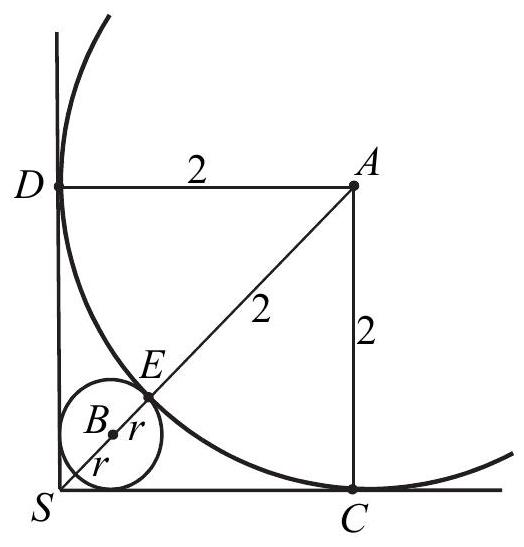
\includegraphics[max width=\textwidth, center]{2025_02_07_a74eed68a1a2147a06fdg-10}

Wtedy $|A S|=2 \sqrt{2}$ oraz $|A E|=2$. Zatem

$$
|S E|=2 \sqrt{2}-2 .
$$

Średnica okręgu o środku $B$ i promieniu $r$ jest krótsza od odcinka $S E$, więc

$$
2 r<2 \sqrt{2}-2, \text { czyli } r<\sqrt{2}-1
$$

Co kończy dowód.

II sposób\\
Przyjmijmy oznaczenia jak na rysunku.\\
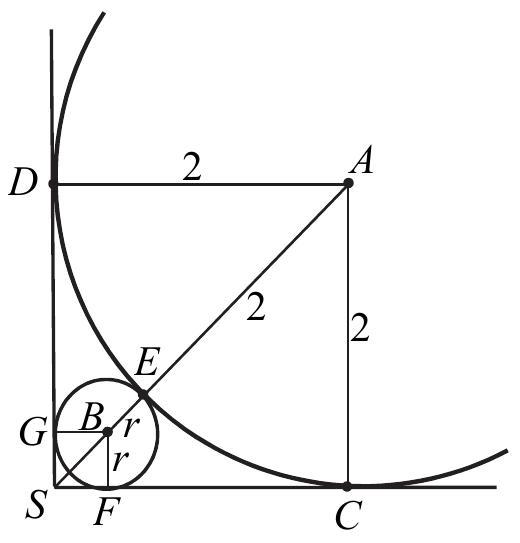
\includegraphics[max width=\textwidth, center]{2025_02_07_a74eed68a1a2147a06fdg-10(1)}

Wtedy $|A S|=2 \sqrt{2},|B S|=r \sqrt{2}$ oraz $|A E|=2$.\\
Ponieważ $|A S|=|B S|+|B E|+|A E|$, więc otrzymujemy

$$
\begin{gathered}
2 \sqrt{2}=r \sqrt{2}+r+2 \\
r(\sqrt{2}+1)=2 \sqrt{2}-2 .
\end{gathered}
$$

Stąd mnożąc obie strony tego równania przez $\sqrt{2}-1$ otrzymujemy

$$
\begin{gathered}
r(\sqrt{2}+1)(\sqrt{2}-1)=2(\sqrt{2}-1)(\sqrt{2}-1) \\
r=2(\sqrt{2}-1)^{2} \\
r=2(2-2 \sqrt{2}+1), \\
r=2(3-2 \sqrt{2}) .
\end{gathered}
$$

Sprawdźmy, czy $2(3-2 \sqrt{2})<\sqrt{2}-1$.\\
Przekształcamy tę nierówność równoważnie.

$$
\begin{aligned}
6-4 \sqrt{2} & <\sqrt{2}-1 \\
7 & <5 \sqrt{2}
\end{aligned}
$$

Ponieważ $\sqrt{2} \approx 1,41>1,4$, więc $5 \sqrt{2}>7$. Oznacza to, że $r<\sqrt{2}-1$.

\section*{Schemat punktowania}
Zdający otrzymuje\\
gdy:

\begin{itemize}
  \item obliczy $|S E|=2 \sqrt{2}-2$\\
albo
  \item zapisze równość $2 \sqrt{2}=r \sqrt{2}+r+2$.\\
i na tym zakończy lub dalej popełni błędy.\\
Zdający otrzymuje 2 p. gdy przeprowadzi pełny dowód.
\end{itemize}

\section*{Uwagi}
\begin{enumerate}
  \item Jeżeli zdający poprawnie obliczy $r$ i zapisze wynik w postaci ułamka, w którym w mianowniku występuje liczba niewymierna, np. $r=\frac{2 \sqrt{2}-2}{\sqrt{2}+1}$, i błędnie szacuje tę liczbę, np. stosując takie same przybliżenia z niedomiarem $\sqrt{2} \mathrm{w}$ liczniku i w mianowniku, to otrzymuje 1 punkt.
  \item Jeżeli zdający błędnie przyjmie, że długość odcinka, którego jednym końcem jest punkt styczności okręgów, a drugim wierzchołek kąta prostego, jest równa długości średnicy mniejszego okręgu i nie wycofa się z tego założenia oraz nie obliczy długości wspomnianego odcinka, to otrzymuje $\mathbf{0}$ punktów.
\end{enumerate}

Zadanie 30. (0-2)\\
II. Wykorzystanie i interpretowanie reprezentacji.\\
4. Funkcje. Zdający szkicuje wykresy funkcji wykładniczych dla różnych podstaw (4.14). Zdający na podstawie wykresu funkcji $y=f(x)$ szkicuje wykresy funkcji $y=f(x+a), y=f(x)+a, y=-f(x)$, $y=f(-x)$ (4.4).

\section*{Przykładowe rozwiązanie}
Ponieważ punkt $P$ leży na wykresie funkcji $f$, więc możemy zapisać:

$$
9=a^{2}, \text { gdzie } a>0 .
$$

Stąd $a=3$.\\
Zbiorem wartości funkcji wykładniczej $f$ jest przedział $(0,+\infty)$. Wykres funkcji $g$ powstaje przez przesunięcie wykresu funkcji $f$ o 2 jednostki w dół. Zatem zbiorem wartości funkcji $g$ jest przedział $(-2,+\infty)$.

\section*{Schemat punktowania}
Zdający otrzymuje\\
gdy:

\begin{itemize}
  \item obliczy $a: a=3$\\
albo
  \item zapisze zbiór wartości funkcji $g$ : $(-2,+\infty)$\\
i na tym zakończy lub dalej popełni błędy.\\
Zdający otrzymuje\\
gdy obliczy $a$ : $a=3$ i zapisze zbiór wartości funkcji $g$ : $(-2,+\infty)$.
\end{itemize}

\section*{Uwaga}
Opis zbioru wartości uznaje się za poprawny, jeśli zbiór ten jest przedstawiony graficznie w sposób jednoznacznie wskazujący, że liczba -2 nie należy do tego zbioru, lub zbiór ten jest opisany słownie, lub jakąkolwiek poprawną nierównością.

\section*{Kryteria uwzględniające specyficzne trudności w uczeniu się matematyki}
Jeśli zdający pomyli porządek liczb na osi liczbowej, np. zapisze zbiór wartości funkcji w postaci $(+\infty,-2)$, to przyznajemy 2 punkty, o ile obliczy $a=3$.

\section*{Zadanie 31. (0-2)}
\begin{center}
\begin{tabular}{l|l}
\begin{tabular}{l}
III. Modelowanie \\
matematyczne. \\
\end{tabular} & \begin{tabular}{l}
5. Ciągi. Zdający stosuje wzór na $n$-ty wyraz i na sumę $n$ \\
początkowych wyrazów ciągu arytmetycznego (5.3). \\
\end{tabular} \\
\hline
\end{tabular}
\end{center}

\section*{Przykładowe rozwiązania}
\section*{I sposób}
Korzystamy ze wzoru na $n$-ty wyraz ciągu arytmetycznego i zapisujemy wzór na $a_{12}$ :

$$
a_{12}=a_{1}+(12-1) \cdot r .
$$

Korzystamy ze wzoru na sumę $n$ początkowych wyrazów ciągu arytmetycznego i zapisujemy wzór na $S_{12}$ :

$$
S_{12}=\frac{2 a_{1}+(12-1) \cdot r}{2} \cdot 12 .
$$

Otrzymujemy układ równań

$$
30=a_{1}+11 r \text { i } 162=12 a_{1}+66 r .
$$

Stąd otrzymujemy

$$
a_{1}=-3 .
$$

\section*{II sposób}
Korzystamy ze wzoru na sumę $n$ początkowych wyrazów ciągu arytmetycznego i zapisujemy wzór na $S_{12}$ :

$$
S_{12}=\frac{a_{1}+a_{12}}{2} \cdot 12 .
$$

Otrzymujemy równanie

$$
162=\frac{a_{1}+30}{2} \cdot 12 .
$$

Stąd otrzymujemy

$$
a_{1}=-3 .
$$

\section*{Schemat punktowania}
\section*{Zdający otrzymuje}
\begin{itemize}
  \item zapisze dwa równania z niewiadomymi $a_{1} \mathrm{i} r$ wynikające z zastosowania poprawnych wzorów na $n$-ty wyraz ciągu arytmetycznego i sumę $n$ początkowych wyrazów ciągu arytmetycznego:\\
np.: $30=a_{1}+11 r$ i $162=\frac{2 a_{1}+11 \cdot r}{2} \cdot 12$\\
albo
  \item zapisze równanie z jedną niewiadomą $a_{1}$ wynikające z zastosowania poprawnego wzoru na sumę $n$ początkowych wyrazów ciągu arytmetycznego bez wykorzystywania różnicy ciągu:\\
np.: $162=\frac{a_{1}+30}{2} \cdot 12$\\
i na tym zakończy lub dalej popełni błędy.
\end{itemize}

\section*{Zdający otrzymuje}
gdy zapisze równanie z jedną niewiadomą $a_{1}$ i obliczy pierwszy wyraz ciągu: $a_{1}=-3$.

\section*{Uwagi}
\begin{enumerate}
  \item Jeżeli zdający, stosując metodę prób i błędów, zapisze poprawny ciąg poprzez wypisanie 12 początkowych kolejnych wyrazów i ustali, że $a_{1}=-3$, to otrzymuje 2 punkty.
  \item Jeżeli zdający, stosując metodę prób i błędów, wypisze co najmniej trzy kolejne wyrazy i ustali, że $a_{1}=-3$, ale nie zapisze wszystkich 12 początkowych wyrazów ciągu, to otrzymuje 1 punkt.
  \item Jeżeli zdający zapisze tylko $a_{1}=-3$ lub $a_{1}=-3$ i $r=3$, to otrzymuje $\mathbf{0}$ punktów.
\end{enumerate}

Zadanie 32. (0-5)

\begin{center}
\begin{tabular}{|l|l|}
\hline
IV. Użycie i tworzenie & \begin{tabular}{l}
8. Geometria na płaszczyźnie kartezjańskiej. Zdający wyznacza \\
równanie prostej przechodzącej przez dwa dane punkty (8.1). \\
Ztrategii. \\
\end{tabular} \\
\begin{tabular}{l}
Zdający wyznacza równanie prostej, która jest równoległa lub \\
prostopadła do prostej danej w postaci kierunkowej i przechodzi \\
przez dany punkt (8.3). Zdający oblicza współrzędne punktu \\
przecięcia dwóch prostych (8.4). \\
\end{tabular} &  \\
\hline
\end{tabular}
\end{center}

\section*{Przykładowe rozwiązania}
I sposób - proste prostopadte\\
Obliczamy współczynnik kierunkowy prostej $A B$

$$
a_{A B}=\frac{1}{3} .
$$

Ponieważ kąt prosty w trójkącie $A B C$ jest przy wierzchołku $B$, więc wyznaczamy równanie prostej prostopadłej do prostej $A B$ i przechodzącej przez punkt $B$

$$
y=-3 x+35
$$

Obliczamy współrzędne punktu $C$, który jest punktem wspólnym prostych określonych równaniami $y=2 x+3$ i $y=-3 x+35$ :

$$
\left\{\begin{array}{l}
y=2 x+3 \\
y=-3 x+35
\end{array}\right.
$$

Stąd po rozwiązaniu układu równań otrzymujemy parę $x=\frac{32}{5}$ i $y=\frac{79}{5}$.\\
Zatem punkt $C$ ma współrzędne. $\left(\frac{32}{5}, \frac{79}{5}\right)$

II sposób - twierdzenie Pitagorasa\\
Ponieważ wierzchołek $C$ trójkąta prostokątnego $A B C$ leży na prostej o równaniu $y=2 x+3$, więc jego współrzędne zapisujemy następująco

$$
C=(x, 2 x+3)
$$

Punkt $B$ jest wierzchołkiem kąta prostego, zatem z twierdzenia Pitagorasa wynika, że

$$
|A C|^{2}=|A B|^{2}+|B C|^{2}
$$

Po podstawieniu współrzędnych punktów $A, B$ i $C$ otrzymujemy równanie

$$
(x-4)^{2}+(2 x+3-3)^{2}=(10-4)^{2}+(5-3)^{2}+(x-10)^{2}+(2 x+3-5)^{2}
$$

czyli równanie

$$
x^{2}-8 x+16+4 x^{2}=36+4+x^{2}-20 x+100+4 x^{2}-8 x+4 .
$$

Zatem

$$
20 x=128 \text { i dalej } x=\frac{32}{5} .
$$

Jeśli $x=\frac{32}{5}$, to $y=\frac{79}{5}$. Zatem $C=\left(\frac{32}{5}, \frac{79}{5}\right)$.

\section*{III sposób - iloczyn skalarny}
Wektory niezerowe są prostopadłe wtedy i tylko wtedy, gdy ich iloczyn skalarny jest równy 0 . W tym przypadku oznacza to, że iloczyn skalarny wektorów $\overrightarrow{A B}$ i $\overrightarrow{B C}$ jest równy 0 .\\
Wspórrzędne wektora $\overrightarrow{A B}$ są równe $\overrightarrow{A B}=[6,2]$.\\
Punkt $C$ ma współrzędne równe $C=(x, 2 x+3)$, więc współ́rzędne wektora $\overrightarrow{B C}$ są równe

$$
\overrightarrow{B C}=[x-10,2 x+3-5] .
$$

Z warunku $\overrightarrow{A B} \circ \overrightarrow{B C}=0$ otrzymujemy równanie

$$
\begin{gathered}
6(x-10)+2(2 x-2)=0, \\
3 x-30+2 x-2=0, \\
x=\frac{32}{5} .
\end{gathered}
$$

Zatem $C=\left(\frac{32}{5}, 2 \cdot \frac{32}{5}+3\right)=\left(\frac{32}{5}, \frac{79}{5}\right)$.

\section*{Schemat punktowania do pełnego rozwiązania \\
 Zdający \\
 - uzależni obie współrzędne punktu $C$ od jednej zmiennej, \\
 $$ \text { np.: } C=(x, 2 x+3) \text { lub } C=\left(\frac{y-3}{2}, y\right) $$}
Rozwiązanie, w którym postęp jest wprawdzie niewielki, ale konieczny na drodze\\
albo

\begin{itemize}
  \item zapisze równość $|A C|^{2}=|A B|^{2}+|B C|^{2}$ i obliczy długość $A B:|A B|=2 \sqrt{10}$,\\
albo
  \item zapisze równość $|A C|^{2}=|A B|^{2}+|B C|^{2}$ i zapisze jedną z długości $|A C|$ lub $|B C|$ w zależności od współrzę̨dnych punktu $C$,\\
albo
  \item obliczy współrzędne wektora $\overrightarrow{A B}: \overrightarrow{A B}=[6,2]$ i zapisze, że $\overrightarrow{A B} \circ \overrightarrow{B C}=0$,\\
albo
  \item wyznaczy współrzędne wektora $\overrightarrow{B C}$ w zależności od współrzędnych punktu $C$ : $\overrightarrow{B C}=[x-10, y-5]$ i zapisze, że $\overrightarrow{A B} \circ \overrightarrow{B C}=0$,\\
albo
  \item wyznaczy współrzędne wektora $\overrightarrow{B C}$ w zależności od jednej współrzędnej punktu $C$, $\mathrm{np} .: \overrightarrow{B C}=[x-10,2 x+3-5]$,\\
albo
  \item obliczy współczynnik kierunkowy równania prostej $A B$ :
\end{itemize}

$$
a_{A B}=\frac{1}{3}
$$

i na tym zakończy lub dalej popełni błędy.\\
Rozwiązanie, w którym jest istotny postęp

\begin{itemize}
  \item wyznaczy współczynnik kierunkowy prostej prostopadłej do prostej $A B$\\
i przechodzącej przez punkt $B: a_{B C}=-3$\\
albo
  \item zapisze równanie z dwiema niewiadomymi, np.:
\end{itemize}

$$
\left(\sqrt{(x-4)^{2}+(y-3)^{2}}\right)^{2}=\left(\sqrt{(10-4)^{2}+(5-3)^{2}}\right)^{2}+\left(\sqrt{(x-10)^{2}+(y-5)^{2}}\right)^{2}
$$

albo

\begin{itemize}
  \item obliczy współrzędne wektora $\overrightarrow{A B}: \overrightarrow{A B}=[6,2]$, wyznaczy współrzędne wektora $\overrightarrow{B C}$ w zależności od jednej wspórłzędnej punktu $C$, np.: $\overrightarrow{B C}=[x-10,2 x+3-5]$ i zapisze, że $\overrightarrow{A B} \circ \overrightarrow{B C}=0$,\\
albo
  \item zapisze równość wynikającą z warunku $\overrightarrow{A B} \circ \overrightarrow{B C}=0$, w której niewiadomymi są dwie współrzędne punktu $C$, np.: $6(x-10)+2(y-5)=0$\\
i na tym zakończy lub dalej popełni błędy.\\
Pokonanie zasadniczych trudności zadania\\
Zdający zapisze równanie z jedną niewiadomą, która jest współrzędną punktu $C, \mathrm{np}$.:
\end{itemize}

$$
2 x+3=-3(x-10)+5
$$

i na tym zakończy lub dalej popełni błędy.\\
Rozwiązanie prawie petne 4 p.\\
Zdający

\begin{itemize}
  \item obliczy $x=\frac{32}{5}$ albo $y=\frac{79}{5}$ i na tym zakończy lub dalej popełni błędy\\
albo
  \item obliczy obie współrzędne punktu $C$ z błędami rachunkowymi.
\end{itemize}

Rozwiązanie petne ....................................................................................................................... 5 p.\\
Zdający obliczy i zapisze współrzędne punktu $C=\left(\frac{32}{5}, \frac{79}{5}\right)$.

\section*{Uwagi}
\begin{enumerate}
  \item Jeżeli zdający realizuje strategię rozwiązania i popełnia jedynie błędy rachunkowe, to może otrzymać 4 punkty, o ile popełnione błędy nie ułatwiają rozważanego zagadnienia na żadnym etapie rozwiązania.
  \item Jeżeli zdający realizuje strategię rozwiązania, ale popełnia błąd, który jednak nie ułatwia rozważanego zagadnienia na żadnym etapie rozwiązania i:\\
a) jedynym błędem merytorycznym w rozwiązaniu jest błąd przy wyznaczaniu współczynnika $a_{A B}$, np. $\frac{x_{A}-x_{B}}{y_{A}-y_{B}}$ zamiast $\frac{y_{A}-y_{B}}{x_{A}-x_{B}}$, to zdający otrzymuje co najwyżej
\end{enumerate}

\section*{3 punkty;}
b) jedynym błędem merytorycznym w rozwiązaniu jest błąd przy wyznaczaniu równania prostej $B C$, to zdający otrzymuje co najwyżej 3 punkty;\\
c) jedynym błędem merytorycznym w rozwiązaniu jest błąd, polegający na tym, że zdający zapisze błędną równość: $|B C|^{2}=|A B|^{2}+|A C|^{2}$, to zdający otrzymuje co najwyżej $\mathbf{3}$ punkty;\\
d) w I sposobie rozwiązania przyjmie, że kąt prosty jest przy wierzchołku A, to otrzymuje co najwyżej $\mathbf{3}$ punkty;\\
e) jedynym błędem merytorycznym w rozwiązaniu jest błąd przy podstawieniu do wzoru na odległość punktów, nawet trzykrotnie powtórzony, to zdający otrzymuje co najwyżej 3 punkty;\\
f) jedynym błędem merytorycznym w rozwiązaniu jest zamiana miejscami współrzędnych punktu $C$ w początkowym etapie rozwiązania, np.: $C=(2 x+3, x)$, to zdający otrzymuje co najwyżej $\mathbf{3}$ punkty;\\
g) jedynym błędem merytorycznym w rozwiązaniu jest przyjęcie bez obliczeń błędnego współczynnika $b$ w równaniu prostej $B C$ (np. $\frac{5}{3}$ ), to zdający otrzymuje co najwyżej 3 punkty.\\
3. Jeżeli zdający realizuje pełną strategię rozwiązania, ale popełnia błąd merytoryczny, który jednak nie ułatwia rozważanego zagadnienia na żadnym etapie rozwiązania i tym jedynym błędem merytorycznym jest błąd, polegający na zastosowaniu nieistniejącego wzoru , $\sqrt{a+b}=\sqrt{a}+\sqrt{b}$ ", to zdający otrzymuje co najwyżej $\mathbf{3}$ punkty.\\
4. Jeżeli zdający popełnia błąd, polegający na tym, że zapisuje błędną równość: $|A B|^{2}=|B C|^{2}+|A C|^{2}$, to otrzymuje co najwyżej 2 punkty.\\
5. Jeżeli zdający wyznaczy równanie prostej prostopadłej do prostej o równaniu $y=2 x+3$, to za rozwiązanie zadania otrzymuje $\mathbf{0}$ punktów, o ile w rozwiązaniu nie występują inne zapisy wymienione w schemacie oceniania, za które należy przyznać zdającemu punkty, np.: $C=(x, 2 x+3)$.\\
6. Jeżeli oprócz poprawnego rozwiązania (kąt prosty przy wierzchołku $B$ ) zdający podaje inne rozwiązanie (np. kąt prosty przy wierzchołku $A$ ), którego nie odrzuca, to otrzymuje co najwyżej 4 punkty.\\
7. Jeżeli zdający zapisze równanie prostej $A B$ w postaci ogólnej (np. dokona właściwego podstawienia współrzędnych punktów do równania prostej przechodzącej przez 2 punkty) i na tym zakończy lub dalej popełnia błędy, to otrzymuje 1 punkt.

Zadanie 33. (0-2)\\
III. Modelowanie matematyczne.\\
10. Elementy statystyki opisowej. Teoria prawdopodobieństwa i kombinatoryka. Zdający oblicza prawdopodobieństwa w prostych sytuacjach, stosując klasyczną definicję prawdopodobieństwa (10.3).

\section*{Przykładowe rozwiązania}
\section*{I sposób}
Zdarzeniem elementarnym jest uporządkowana para $(x, y)$, gdzie $x \in A$ i $y \in B$. Zatem zbiór wszystkich zdarzeń elementarnych ma postać:

$$
\begin{aligned}
\Omega=\{ & (100,10),(100,11),(100,12),(100,13),(100,14),(100,15),(100,16), \\
& (200,10),(200,11),(200,12),(200,13),(200,14),(200,15),(200,16), \\
& (300,10),(300,11),(300,12),(300,13),(300,14),(300,15),(300,16), \\
& (400,10),(400,11),(400,12),(400,13),(400,14),(400,15),(400,16), \\
& (500,10),(500,11),(500,12),(500,13),(500,14),(500,15),(500,16), \\
& (600,10),(600,11),(600,12),(600,13),(600,14),(600,15),(600,16), \\
& (700,10),(700,11),(700,12),(700,13),(700,14),(700,15),(700,16)\} .
\end{aligned}
$$

Liczba wszystkich zdarzeń elementarnych jest równa $|\Omega|=7 \cdot 7=49$.\\
Niech $A$ oznacza zdarzenie polegające na tym, że suma wylosowanych liczb będzie podzielna przez 3 . $Z$ cechy podzielności liczby całkowitej przez 3 wynika, że suma cyfr otrzymanej liczby $x+y$ musi być podzielna przez 3 . Zbiór $A$ ma postać:

$$
\begin{aligned}
A=\{ & (100,11),(100,14),(200,10),(200,13),(200,16), \\
& (300,12),(300,15),(400,11),(400,14),(500,10), \\
& (500,13),(500,16),(600,12),(600,15),(700,11),(700,14)\} .
\end{aligned}
$$

Zdarzeniu $A$ sprzyja więc 16 zdarzeń elementarnych, czyli $|A|=16$.\\
Prawdopodobieństwo zdarzenia $A$ jest równe

$$
P(A)=\frac{|A|}{|\Omega|}=\frac{16}{49} .
$$

Odpowiedź: Prawdopodobieństwo zdarzenia polegającego na tym, że suma wylosowanych liczb będzie liczbą podzielną przez 3, jest równe $\frac{16}{49}$.

\section*{Uwaga}
Zdający może zapisać zbiór wszystkich zdarzeń elementarnych jako zbiór sum możliwych do utworzenia w wyniku losowania, tzn. może zastosować zapis:

$$
\begin{aligned}
\Omega=\{ & \{110,111,112,113,114,115,116, \\
& 210,211,212,213,214,215,216, \\
& 310,311,312,313,314,315,316, \\
& 410,411,412,413,414,415,416, \\
& 510,511,512,513,514,515,516, \\
& 610,611,612,613,614,615,616, \\
& 710,711,712,713,714,715,716\} .
\end{aligned}
$$

Wtedy zbiór\\
$A=\{111,114,210,213,216,312,315,411,414,510,513,516,612,615,711,714\}$.

II sposób\\
Rysujemy tabelę, która przedstawia model rozważanego doświadczenia.

\begin{center}
\begin{tabular}{|c|c|c|c|c|c|c|c|}
\hline
 & 100 & 200 & 300 & 400 & 500 & 600 & 700 \\
\hline
10 &  & $\times$ &  &  & $\times$ &  &  \\
\hline
11 & $\times$ &  &  & X &  &  & $\times$ \\
\hline
12 &  &  & X &  &  & $\times$ &  \\
\hline
13 &  & $\times$ &  &  & $\times$ &  &  \\
\hline
14 & $\times$ &  &  & $\times$ &  &  & $\times$ \\
\hline
15 &  &  & $\times$ &  &  & $\times$ &  \\
\hline
16 &  & $\times$ &  &  & $\times$ &  &  \\
\hline
\end{tabular}
\end{center}

Zdarzeniom elementarnym odpowiadają komórki tej tabeli. Jest ich 49, zatem $|\Omega|=49$.\\
Symbolem $\times$ zaznaczamy te zdarzenia elementarne, które sprzyjają zdarzeniu $A$, polegającemu na tym, że suma wylosowanych liczb jest podzielna przez 3.\\
Zdarzeniu $A$ sprzyja więc 16 zdarzeń elementarnych, czyli $|A|=16$.\\
Prawdopodobieństwo zdarzenia $A$ jest równe

$$
P(A)=\frac{|A|}{|\Omega|}=\frac{16}{49} .
$$

Odpowiedź: Prawdopodobieństwo zdarzenia polegającego na tym, że suma wylosowanych liczb będzie liczbą podzielną przez 3 , jest równe $\frac{16}{49}$.

\section*{III sposób}
Rysujemy drzewko rozważanego doświadczenia.\\
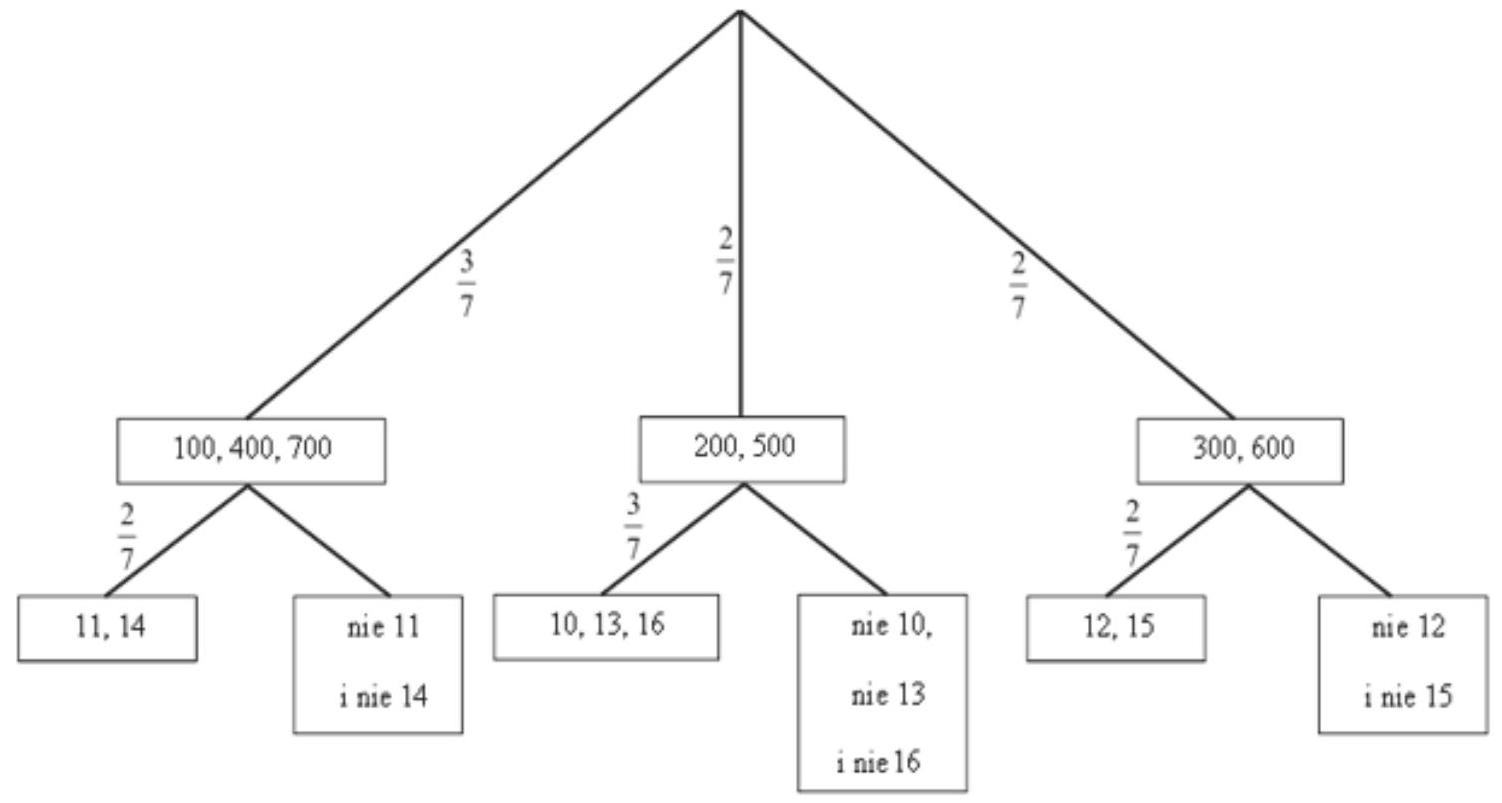
\includegraphics[max width=\textwidth, center]{2025_02_07_a74eed68a1a2147a06fdg-20}

Prawdopodobieństwo zdarzenia $A$ jest równe

$$
P(A)=\frac{3}{7} \cdot \frac{2}{7}+\frac{2}{7} \cdot \frac{3}{7}+\frac{2}{7} \cdot \frac{2}{7}=\frac{16}{49} .
$$

Odpowiedź: Prawdopodobieństwo zdarzenia polegającego na tym, że suma wylosowanych liczb będzie liczbą podzielną przez 3, jest równe $\frac{16}{49}$.

\section*{Uwaga}
Zdający może narysować drzewo probabilistyczne, w którym na każdym z etapów lub na jednym z etapów rozważa każdą możliwą do wylosowania liczbę oddzielnie. Przykład takiego drzewa znajduje się poniżej.\\
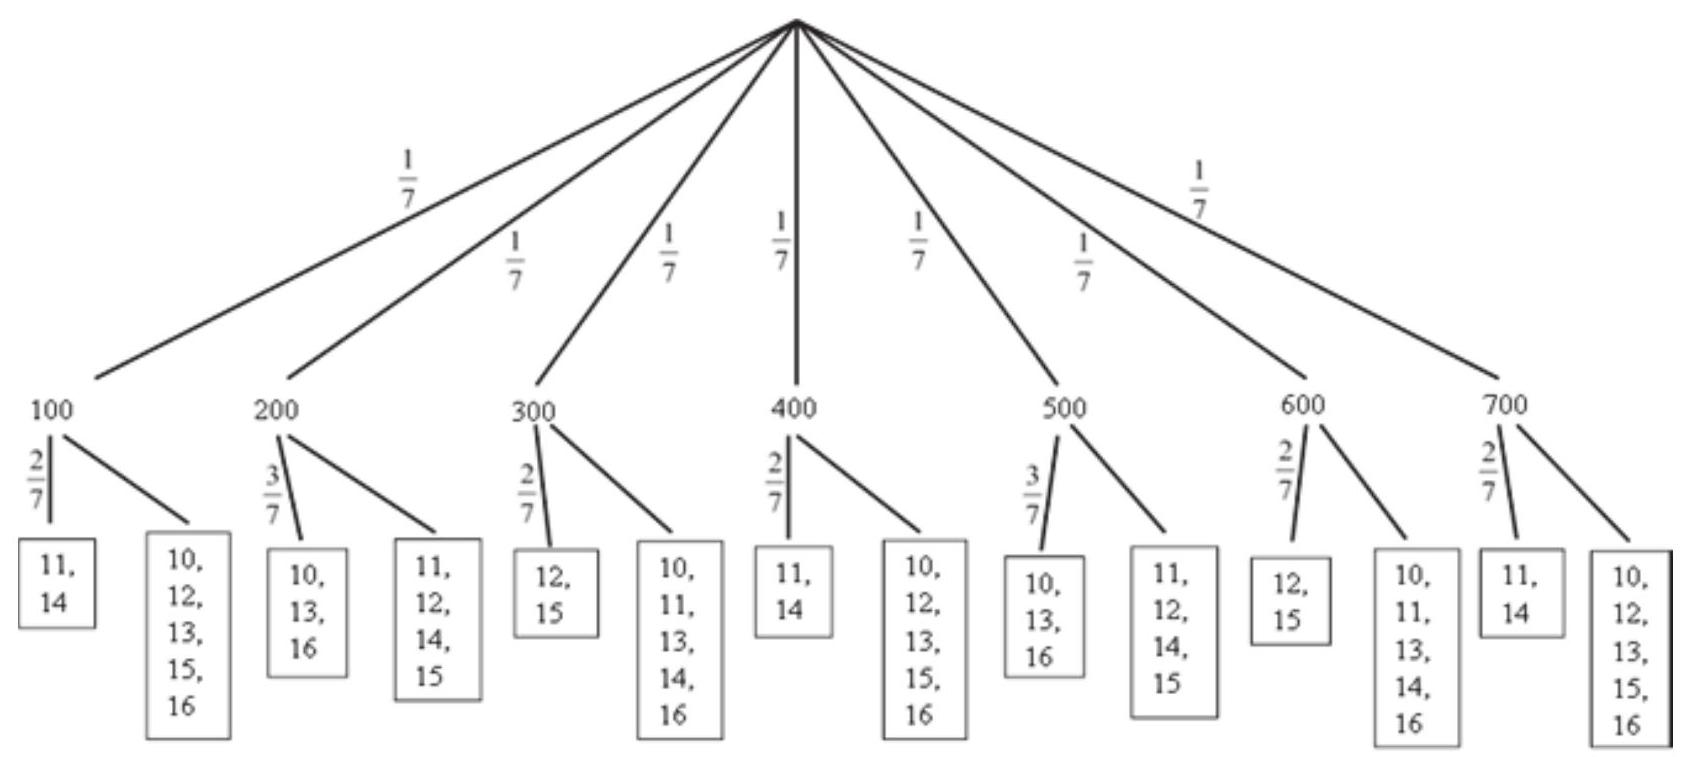
\includegraphics[max width=\textwidth, center]{2025_02_07_a74eed68a1a2147a06fdg-20(1)}

Prawdopodobieństwo zdarzenia $A$ może być obliczone w następujący sposób:

$$
P(A)=5 \cdot \frac{1}{7} \cdot \frac{2}{7}+2 \cdot \frac{1}{7} \cdot \frac{3}{7}=\frac{16}{49} .
$$

\section*{Schemat punktowania}
Rozwiązanie, w którym postęp jest niewielki, ale konieczny na drodze do pełnego rozwiązania 1 p. Zdający

\begin{itemize}
  \item zapisze, że $|\Omega|=7.7$\\
albo
  \item zapisze, że suma cyfr utworzonej sumy wylosowanych liczb musi być podzielna przez 3,\\
albo
  \item poda sposób obliczania $|A|$, np. przyjmie porządek przy wyznaczaniu sum podzielnych przez 3 oraz wyznaczy przynajmniej 4 zdarzenia elementarne sprzyjające zdarzeniu $A$ i nie zaliczy do zbioru $A$ niewłaściwego zdarzenia elementarnego,\\
albo
  \item przedstawi graficznie model doświadczenia z 49 zdarzeniami elementarnymi, np. narysuje tabelę z 7 kolumnami i 7 wierszami,\\
albo
  \item narysuje drzewko doświadczenia:
\end{itemize}

\begin{enumerate}
  \item składające się ze wszystkich 49 gałęzi\\
albo
  \item składające się z mniej niż 49 gałęzi, ale wskaże na nim gałęzie odpowiadające wylosowaniu w pierwszym etapie dwóch spośród 7 liczb: 100, 200, 300, 400, 500, 600, 700 oraz wylosowaniu w drugim etapie odpowiednich liczb dających z liczbą wylosowaną w pierwszym etapie sumę podzielną przez 3\\
i na tym zakończy lub dalej popełni błędy.
\end{enumerate}

\section*{Rozwiązanie, w którym jest istotny postęp}
\section*{Zdający}
\begin{itemize}
  \item zapisze wszystkie zdarzenia elementarne sprzyjające zdarzeniu $A$\\
albo
  \item zapisze, że $|\Omega|=7.7$ i zapisze, że suma cyff utworzonej sumy wylosowanych liczb musi być podzielna przez 3,\\
albo
  \item zapisze, że $|\Omega|=7.7$ i poda sposób obliczania $|A|$, np. przyjmie porządek przy wyznaczaniu sum podzielnych przez 3, wyznaczy przynajmniej 4 zdarzenia elementarne sprzyjające zdarzeniu $A$, ale nie zaliczy do zbioru $A$ niewłaściwego zdarzenia elementarnego,\\
albo
  \item przedstawi graficznie model doświadczenia z 49 zdarzeniami elementarnymi, np. narysuje tabelę z 7 kolumnami i 7 wierszami oraz zapisze, że $|\Omega|=7 \cdot 7$,\\
albo
  \item narysuje drzewko doświadczenia:
\end{itemize}

\begin{enumerate}
  \item składające się ze wszystkich 49 gałęzi i zapisze prawdopodobieństwa na co najmniej jednym odcinku każdego $z$ etapów\\
albo
  \item składające się z mniej niż 49 gałęzi, ale wskaże na nim gałęzie odpowiadające wylosowaniu w pierwszym etapie dwóch spośród 7 liczb: 100, 200, 300, 400, 500, 600, 700 oraz wylosowaniu w drugim etapie odpowiednich liczb dających z liczbą wylosowaną $w$ pierwszym etapie sumę podzielną przez 3 i zapisze prawdopodobieństwa na co najmniej jednym odcinku każdego z etapów;\\
albo
\end{enumerate}

\begin{itemize}
  \item narysuje drzewko doświadczenia, w którym wskaże wszystkie gałęzie odpowiadające zdarzeniu $A$\\
i na tym zakończy lub dalej popełni błędy.
\end{itemize}

\section*{Pokonanie zasadniczych trudności zadania 3 p. Zdający}
\begin{itemize}
  \item zapisze, że $|\Omega|=7.7$ oraz zapisze wszystkie zdarzenia elementarne sprzyjające zdarzeniu $A$, ale nie zaliczy do zbioru $A$ niewłaściwego zdarzenia elementarnego\\
albo
  \item zapisze, że $|\Omega|=7.7$ oraz zapisze, że $|A|=16$ i przedstawi sposób obliczenia tej liczby, np. zapisze, że suma cyfr utworzonej sumy wylosowanych liczb musi być podzielna przez 3 i wskaże w dowolny sposób przykładowe zdarzenie elementarne lub przyjmie porządek przy wyznaczaniu sum podzielnych przez 3 i wyznaczy przynajmniej 4 zdarzenia elementarne sprzyjające zdarzeniu $A$, ale nie zaliczy do zbioru $A$ niewłaściwego zdarzenia elementarnego,\\
albo
  \item przedstawi graficznie model doświadczenia z 49 zdarzeniami elementarnymi (np. narysuje tabelę z 7 kolumnami i 7 wierszami), zapisze $|\Omega|=7 \cdot 7$, oraz zaznaczy 16 zdarzeń elementarnych sprzyjających zdarzeniu $A$ i żadnych innych zdarzeń elementarnych nie zaliczy do $A$,\\
albo
  \item narysuje drzewko doświadczenia, w którym wystąpią wszystkie gałęzie odpowiadające zdarzeniu $A$ wraz z prawdopodobieństwami oraz poprawnie zastosuje regułę drzewka do obliczenia prawdopodobieństwa $P(A)$\\
i na tym zakończy lub dalej popełni błędy.
\end{itemize}

\section*{Rozwiązanie pełne}
Zdający obliczy prawdopodobieństwo zdarzenia $A: P(A)=\frac{|A|}{|\Omega|}=\frac{16}{49}$.

\section*{Uwagi}
\begin{enumerate}
  \item Jeżeli zdający uzyska w wyniku końcowym liczbę spoza przedziału $\langle 0,1\rangle$, to może otrzymać co najwyżej 2 punkty.
  \item Jeżeli zdający w swoim rozwiązaniu wypisze 17 zdarzeń elementarnych sprzyjających zdarzeniu $A$, w tym 16 poprawnych i jedno niepoprawne oraz otrzyma prawdopodobieństwo równe $\frac{17}{49}$, to otrzymuje 2 punkty.
  \item Jeżeli zdający w swoim rozwiązaniu wypisze 15 poprawnych zdarzeń elementarnych sprzyjających zdarzeniu $A$ i otrzyma prawdopodobieństwo równe $\frac{15}{49}$, to otrzymuje 2 punkty.
  \item Jeżeli zdający w swoim rozwiązaniu przyjmie błędną liczbę wszystkich zdarzeń elementarnych i nie jest to efekt błędu rachunkowego, np. przyjmie $|\Omega|=7 \cdot 6$, to może otrzymać co najwyżej 2 punkty.
  \item Jeżeli zdający w swoim rozwiązaniu zapisze jedynie $|\Omega|=7 \cdot 7,|A|=16$ i nie przedstawi czytelnego uzasadnienia liczby zdarzeń elementarnych sprzyjających zdarzeniu $A$, i obliczy $P(A)=\frac{|A|}{|\Omega|}=\frac{16}{49}$, to otrzymuje 1 punkt.
  \item Jeżeli zdający w swoim rozwiązaniu zapisze $|\Omega|=7 \cdot 7,|A|=16$ oraz zapisze, że suma cyfr utworzonej sumy wylosowanych liczb musi być podzielna przez3, ale wprzedstawionym rozwiązaniu nie można zidentyfikować żadnego zdarzenia elementarnego, które zdający powinien rozważać, to otrzymuje 2 punkty, nawet jeśli w rozwiązaniu występuje poprawny wynik końcowy.
  \item Jeżeli zdający w swoim rozwiązaniu wypisze 16 zdarzeń elementarnych sprzyjających zdarzeniu $A$, w tym 15 poprawnych i jedno niewłaściwe i konsekwentnie rozwiąże zadanie do końca, to otrzymuje 2 punkty.
\end{enumerate}

Zadanie 34. (0-4)\\
IV. Użycie i tworzenie strategii.

G11. Bryły. Zdający oblicza pole powierzchni i objętość graniastosłupa prostego (G11.2).\\
3. Równania i nierówności. Zdający rozwiązuje równania kwadratowe z jedną niewiadomą (3.4).

\section*{Przykładowe rozwiązanie}
Przyjmijmy oznaczenia jak na rysunku.\\
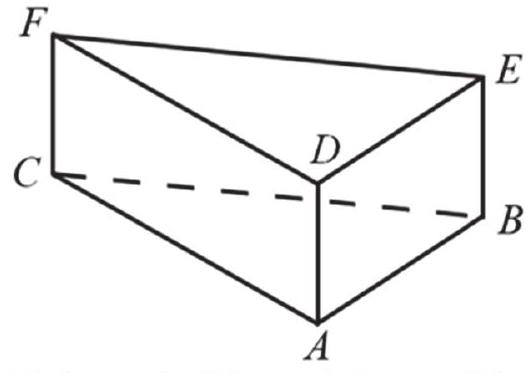
\includegraphics[max width=\textwidth, center]{2025_02_07_a74eed68a1a2147a06fdg-23}

Rozważany graniastosłup ma 5 ścian, a każda z nich ma takie samo pole. Obliczamy pole podstawy, a zarazem pole jednej ściany bocznej:

$$
45 \sqrt{3}: 5=9 \sqrt{3} .
$$

Podstawą graniastosłupa jest trójkąt równoboczny, więc jego pole jest równe

$$
P_{A B C}=\frac{a^{2} \sqrt{3}}{4} .
$$

Obliczamy długość krawędzi podstawy:

$$
\begin{gathered}
\frac{a^{2} \sqrt{3}}{4}=9 \sqrt{3}, \\
a=6 .
\end{gathered}
$$

Ściana boczna jest prostokątem o bokach długości $a$ i $h$, więc pole każdej ściany bocznej jest równe

$$
P_{A B E D}=a h .
$$

Z warunków zadania wynika, że:

$$
a h=9 \sqrt{3} .
$$

Znamy długość krawędzi podstawy $a$, zatem:

$$
6 h=9 \sqrt{3} .
$$

Obliczamy wysokość graniastosłupa

$$
h=\frac{3}{2} \sqrt{3} .
$$

Objętość graniastosłupa jest równa

$$
V=P_{A B C} \cdot h=9 \sqrt{3} \cdot \frac{3 \sqrt{3}}{2}=\frac{81}{2} .
$$

\section*{Schemat punktowania}
Rozwiązanie, w którym postęp jest niewielki, ale konieczny na drodze do pełnego rozwiązania zadania\\
Zdający

\begin{itemize}
  \item zapisze zależność między wielkościami $a$ i $h$ wynikającą z równości pól podstawy i ściany bocznej graniastosłupa: $\frac{a^{2} \sqrt{3}}{4}=a h$\\
albo
  \item obliczy pole jednej ściany graniastosłupa: $45 \sqrt{3}: 5=9 \sqrt{3}$,\\
albo
  \item zapisze równanie: $2 \cdot \frac{a^{2} \sqrt{3}}{4}+3 a h=45 \sqrt{3}$\\
albo
  \item zapisze równania: $2 \cdot \frac{1}{2} a h_{p}+3 a h=45 \sqrt{3} \mathrm{i} \frac{1}{2} a h_{p}=a h$ i na tym zakończy lub dalej popełni błędy.
\end{itemize}

Rozwiązanie, w którym jest istotny postęp 2 p.\\
Zdający

\begin{itemize}
  \item zapisze równanie z jedną niewiadomą, pozwalające na wyznaczenie długości krawędzi podstawy lub wysokości graniastosłupa i na tym zakończy lub dalej popełni błędy\\
albo
  \item uzależni objętość bryły od jednej zmiennej\\
i na tym zakończy lub dalej popełni błędy.
\end{itemize}

\section*{Pokonanie zasadniczych trudności zadania}
Zdający

\begin{itemize}
  \item obliczy długość krawędzi podstawy i wysokość graniastosłupa: $a=6, h=\frac{3}{2} \sqrt{3}$\\
albo
  \item obliczy długość krawędzi podstawy graniastosłupa: $a=6$ i uzależni objętość bryły od jednej zmiennej a lub obliczy wysokość graniastosłupa $h=\frac{3}{2} \sqrt{3}$ i uzależni objętość bryły od jednej zmiennej $h$ i na tym zakończy lub dalej popełni błędy.
\end{itemize}

\section*{Rozwiązanie pełne}
Zdający obliczy objętość graniastosłupa: $V=\frac{81}{2}$.

\section*{Uwagi}
\begin{enumerate}
  \item Jeżeli zdający realizuje strategię rozwiązania, a jedynymi błędami w przedstawionym rozwiązaniu są błędy rachunkowe, to otrzymuje 3 punkty.
  \item Jeżeli zdający popełnia błąd polegający na niepoprawnym stosowaniu wzoru na pole trójkąta równobocznego albo wzoru na pole prostokąta, to otrzymuje 2 punkty, o ile nie popełnia innych błędów i rozwiąże zadanie do końca.
  \item Jeżeli zdający popełnia błąd, polegający na niewłaściwym określeniu zależności między polem podstawy a polem ściany bocznej i w efekcie rozważa jeden z trzech przypadków: $2 P_{p}=P_{s b}, P_{p}=3 P_{s b}, 2 P_{p}=3 P_{s b}$, albo błąd, polegający na przyjęciu, że graniastosłup ma trzy ściany boczne i jedną podstawę, to otrzymuje 2 punkty, o ile nie popełnia innych błędów i rozwiąże zadanie do końca.
  \item Jeżeli zdający popełnia jeden błąd, opisany w uwagach 2. lub 3., a ponadto popełnia błędy rachunkowe, ale poprawnie obliczy pole jednej ściany albo realizuje strategię rozwiązania, to otrzymuje co najwyżej 1 punkt.
  \item Jeżeli zdający popełnia inne niż wymienione w uwagach 2 . lub 3 . błędy, dotyczące pól ścian bryły, ale poprawnie obliczy pole jednej ściany albo realizuje strategię rozwiązania, to otrzymuje co najwyżej 1 punkt.
  \item Jeżeli zdający rozważa graniastosłup trójkątny, który nie jest prawidłowy, to może otrzymać co najwyżej 1 punkt.
\end{enumerate}

\end{document}